\documentclass[../ManualeSviluppatore.tex]{subfiles}

\begin{document}
\section{Per iniziare}

	Nel caso in cui si voglia utilizzare o estendere il codice di CLIPS si consiglia di seguire i passi di seguito descritti. Le procedure descritte valgono sia per computer con sistema operativo \textbf{Microsoft Windows 10} sia con \textbf{Linux Ubuntu 16.04}.

	\subsection{IDE}
		È consigliato aprire ed eventualmente modificare il progetto con l'IDE \gls{Android Studio}, ossia l'IDE utilizzato ufficialmente nello sviluppo. La versione con cui è stato sviluppato il progetto è la 1.5.1. Questa sezione farà riferimento a tale versione.
		
	 \gls{Android Studio} è disponibile gratuitamente al seguente link:
		\begin{quote}
			\centering
			\url{http://developer.android.com/sdk/index.html}
		\end{quote}
		
		\paragraph*{Nota:} 
			Il progetto non è stato provato su \gls{Android Studio} con versioni successive o precedenti, non dovrebbe portare elevate differenze per le versioni successive.
		
		
		
		
	\subsection{Download del progetto}
		\paragraph*{}
			Per poter accedere al codice è necessario accedere al link:
		\begin{quote}
			\centering
			\url{https://github.com/LeafSWE/clips}
		\end{quote}

		\paragraph*{}
			Successivamente selezionare il branch \textbf{master} e cliccare \textbf{DOWNLOAD ZIP} e \textbf{SALVA}:
			
			\begin{figure} [h]
				\centering
				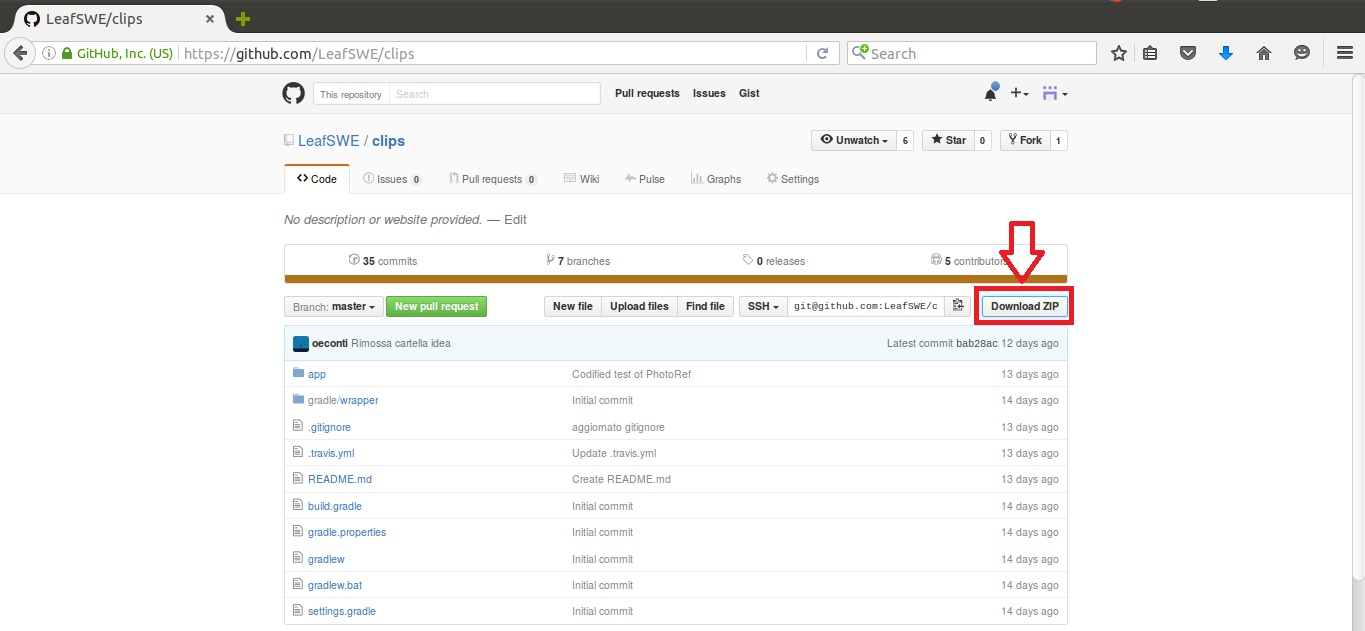
\includegraphics[width=\textwidth]{img/DownloadZip}
				\caption{Download progetto da Github}
				\label{fig:DownloadZip}
			\end{figure}
			
			\begin{figure} [h]
				\centering
				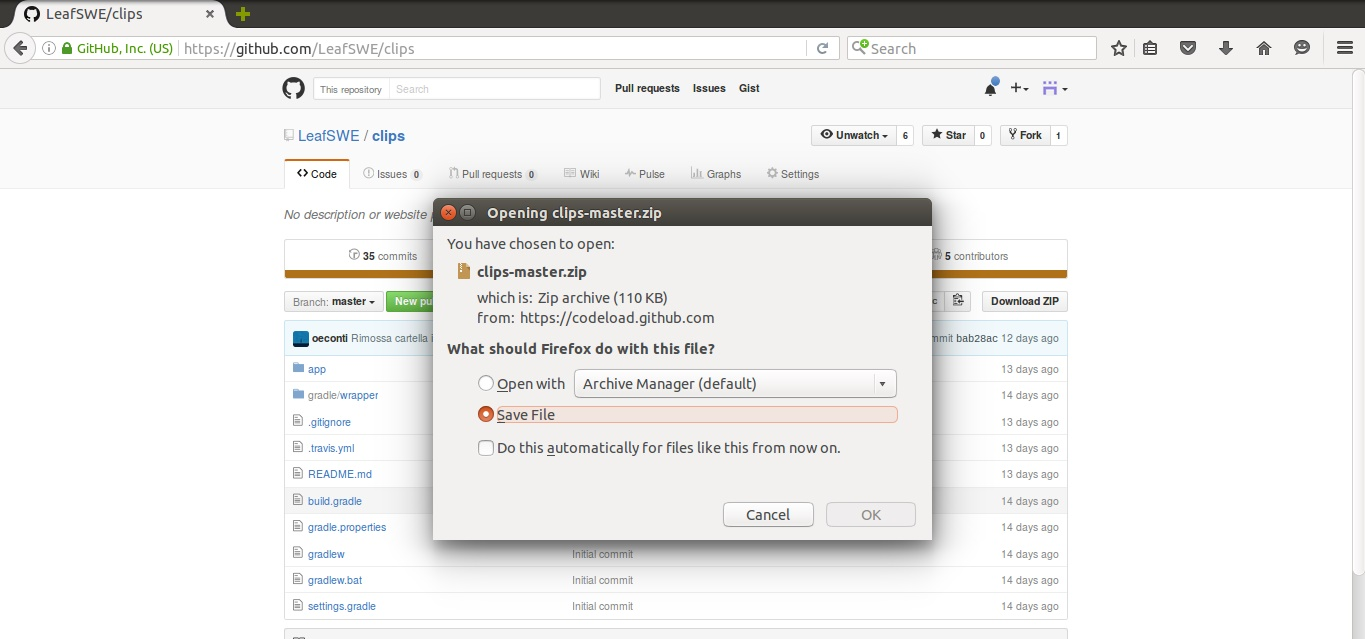
\includegraphics[width=\textwidth]{img/Download}
				\caption{Download file progetto da Github}
				\label{fig:DownloadZip2}
			\end{figure}
			
		\paragraph*{}
			Scaricato il file \verb|clips-master.zip| estrarlo con il tool per l'estrazione file preferito:
			
			\begin{figure} [h]
				\centering
				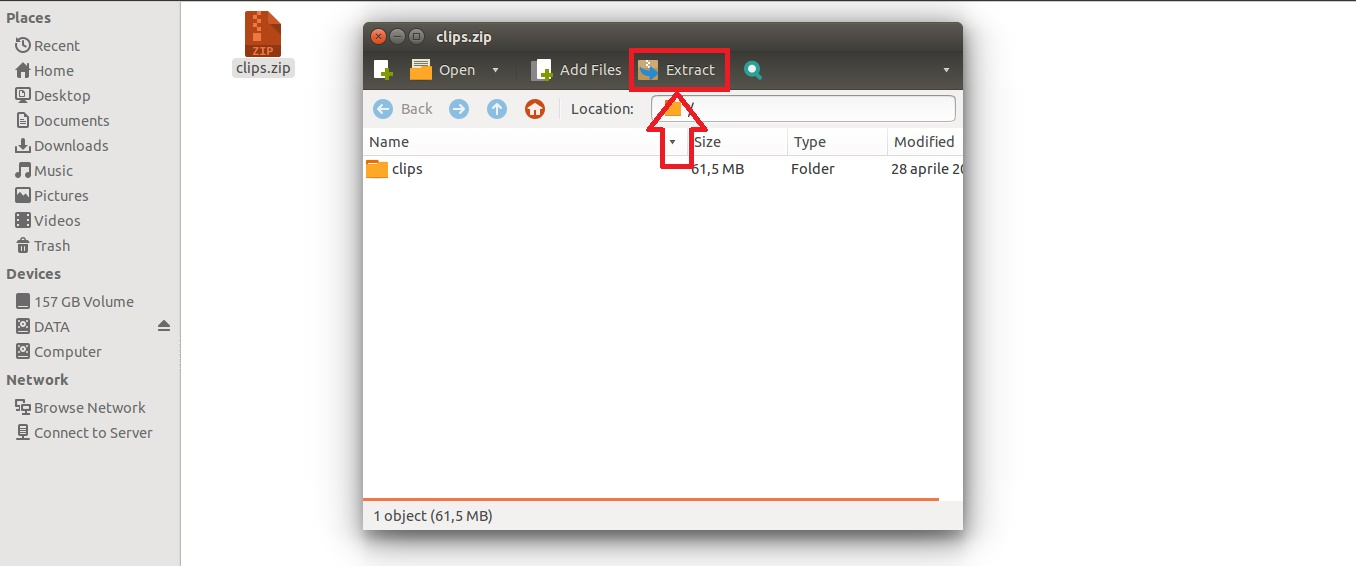
\includegraphics[width=\textwidth]{img/EstraiZip}
				\caption{Estrazione file zip}
				\label{fig:EstraiZip}
			\end{figure}
			
			
		
	\newpage	
	\subsection{Aprire il progetto con \gls{Android} Studio}
		Aprire \gls{Android Studio} e selezionare \textbf{Opening an existing \gls{Android Studio}\ 
project}:
		
		\begin{figure} [h]
			\centering
			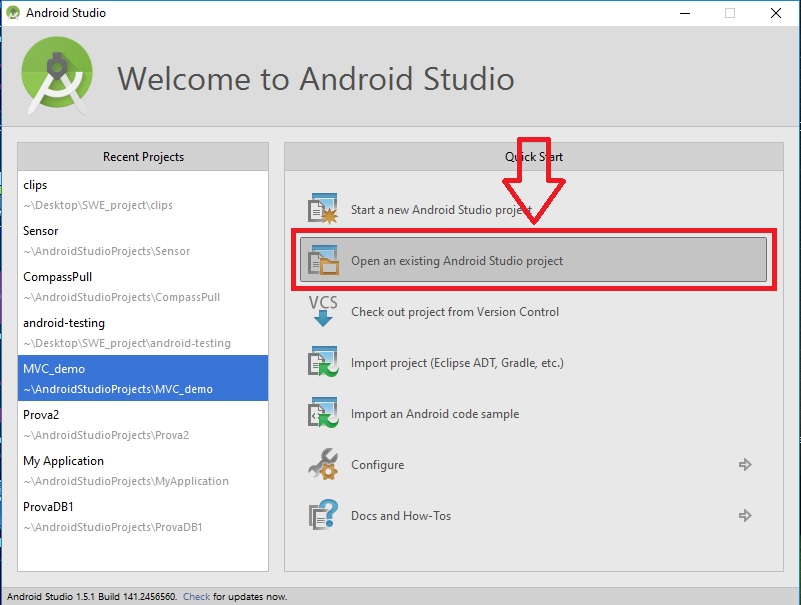
\includegraphics[scale=0.5]{img/AprireProgetto}
			\caption{Aprire il progetto con \gls{Android} Studio}
			\label{fig:AprireProgetto}
		\end{figure}
		
		\paragraph*{}
			Selezionare, seguendo il giusto path, la cartella del progetto \verb|clips-master|. Attendere la \textbf{Build project info} di Gradle. Anche quando \gls{Android Studio} è aperto attendere la conclusione del processo di Gradle:
			
		\begin{figure} [h]
			\centering
			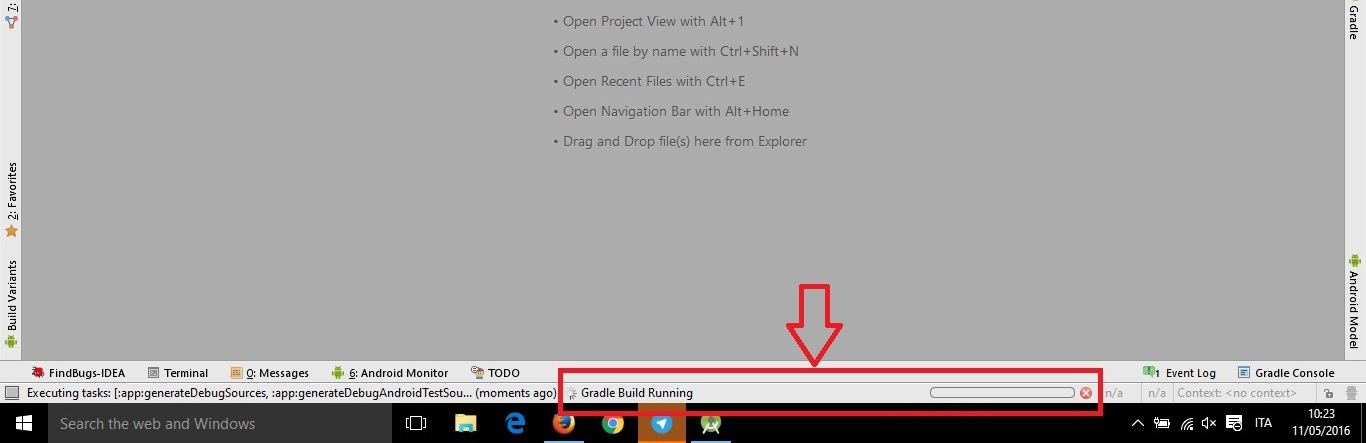
\includegraphics[width=\textwidth]{img/BuildGradleCut}
			\caption{Build project info di Gradle}
			\label{fig:BuildGradleCut}
		\end{figure}
		
		\paragraph*{Nota:}
			Nel caso in cui il processo di Gradle fallisca, come in figura \ref{fig:GradleError}, seguire le indicazioni nella sezione successiva \ref{subsec:ConfigGradleAS}
			
		\begin{figure} [h]
			\centering
			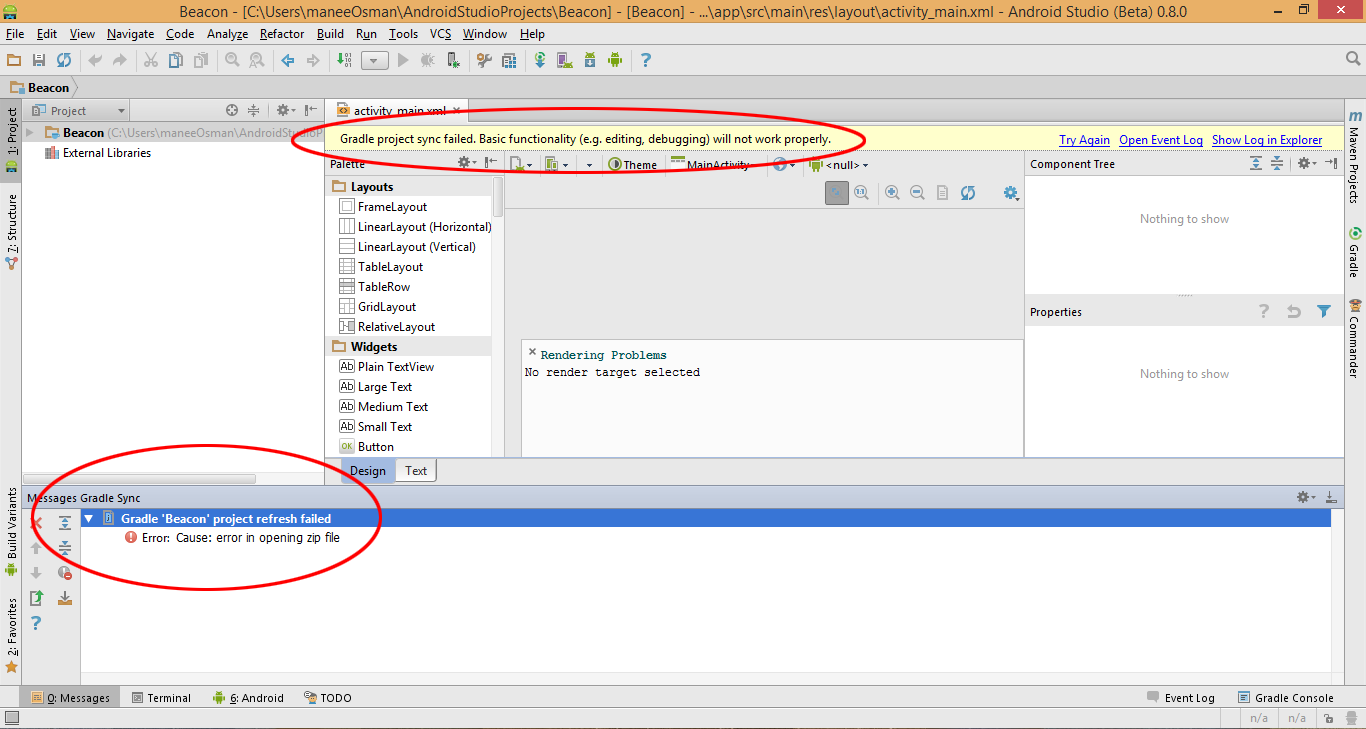
\includegraphics[width=\textwidth]{img/GradleError}
			\caption{Errore build project info di Gradle}
			\label{fig:GradleError}
		\end{figure}
		
		\newpage
		\subsection{Configurazione Gradle in \gls{Android} Studio}
		\label{subsec:ConfigGradleAS}
			Per assicurarsi che la \textbf{build} di Gradle funzioni correttamente: in \gls{Android Studio} cliccare \textbf{File} $\rightarrow$ \textbf{Settings} oppure premere \textbf{CTRL+ALT+S}:
			
		
		\begin{figure} [h]
			\centering
			\includegraphics[width=\textwidth]{img/settings}
			\caption{Aprire le impostazioni \gls{Android} Studio}
			\label{fig:Settings}
		\end{figure}
		
		\paragraph*{}
			Nella nuova finestra aperta spostarsi su \textbf{Build, Execution, Deployment} $\rightarrow$ \textbf{Build Tools} $\rightarrow$ \textbf{Gradle}. Spuntare l'opzione \textbf{Use default gradle \gls{Wrapper} (reccomended)} come in figura \ref{fig:SetGradle}:
			
			\begin{figure} [h]
				\centering
				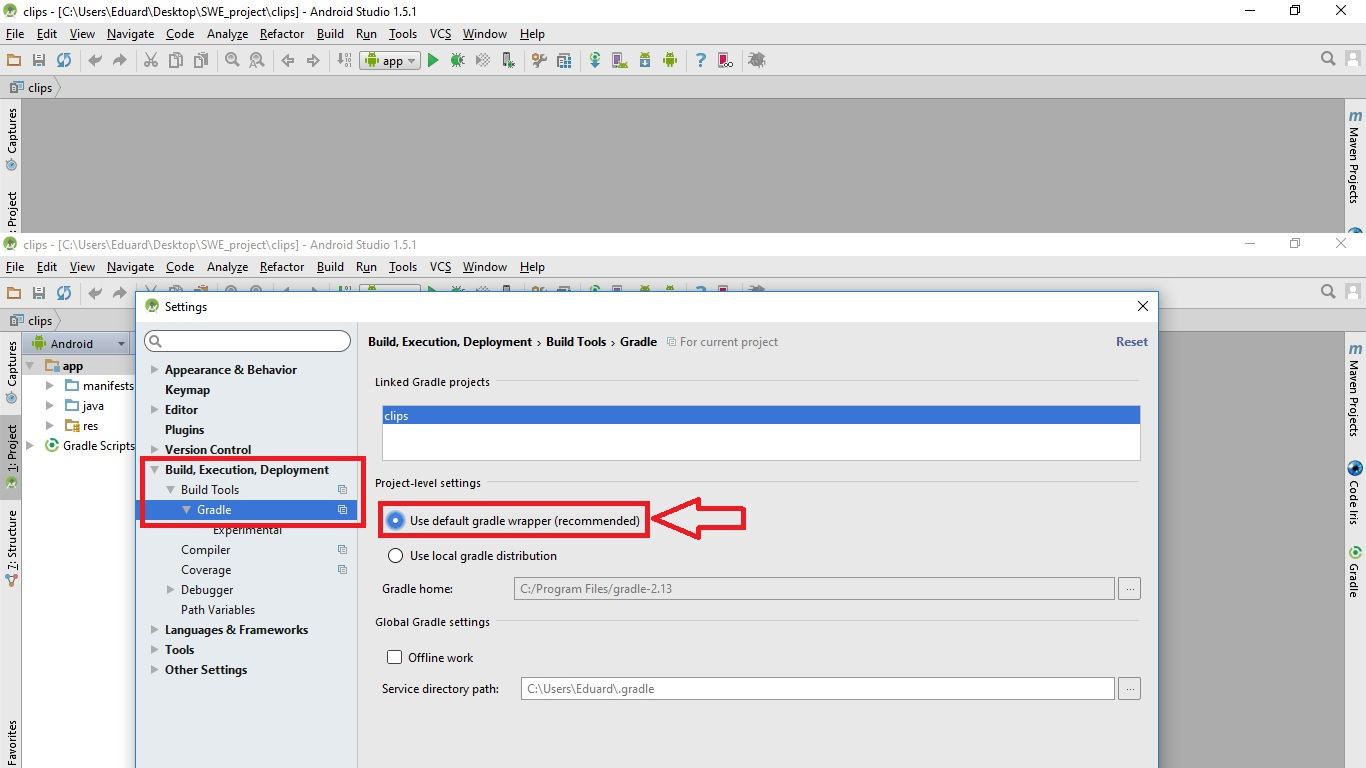
\includegraphics[width=\textwidth]{img/SetGradle}
				\caption{Impostare Gradle correttamente}
				\label{fig:SetGradle}
			\end{figure}
		

\end{document}